%Doc class
\documentclass[a4paper,12pt,oneside, utf8x]{report} 
%Packages
\usepackage[UTF8, scheme = plain]{ctex}
\usepackage[ %Bibliography
  backend   = bibtex,
  sortcites = true,
  sorting   = nty,
  style     = ieee
  ]{biblatex}
\usepackage{geometry}
\usepackage{longtable} %for tables
\usepackage{textcomp}
\usepackage{gensymb}
\usepackage{mathptmx}
\usepackage{graphicx}
\usepackage{float}
\usepackage{setspace}
\usepackage[title,titletoc,toc]{appendix}
\usepackage{enumitem}
\usepackage{caption}
\usepackage{subcaption}
\usepackage{amsmath}
\usepackage{tocloft}
\usepackage{titlesec}
\usepackage{parskip}
\usepackage[format=plain,font=it]{caption}

\renewcommand\cftfigpresnum{Figure }
\renewcommand\cftfigaftersnum{.}
\addtolength{\cftfignumwidth}{35pt}
\renewcommand\cfttabpresnum{Table }
\renewcommand\cfttabaftersnum{.}
\addtolength{\cfttabnumwidth}{27pt}
\emergencystretch=1em

\usepackage{url}
\urlstyle{same}

%Bibliography loading
\addbibresource{ref.bib}

%Formatting
\geometry{a4paper, top = 1in, bottom = 1in, left = 1.5in, right = 1in,}
\titleformat{\chapter}[display]{\bfseries\centering}{\LARGE Chapter \thechapter}{-0.5em}{\LARGE}
\titleformat{\section}{\Large\bfseries}{\thesection}{1em}{}
\titleformat{\subsection}{\large\bfseries}{\thesubsection}{1em}{}
\titlespacing*{\chapter}{0pt}{*4}{*1.5}


%TEXT SHORTCUTS
\newcommand{\projfull}{Exploring Possibilities in Incorporating Blockchain-based Distributed Ledgers in Rapid Transit Automated Fare Collection (AFC) Backend}

%GRAPHICS
\graphicspath{{figures/}}

\begin{document}
\linespread{1.6}\selectfont

%------------------Acknowledgement----------------
\begin{titlepage}
\pagestyle{empty}
    \hfill \break \hfill \break
    {{\huge \centering \textbf{Acknowledgement}\par}
    \hfill \break \hfill \break
    --acknowledgement page--

    }
\end{titlepage}

%------------------ABSTRACT PAGE------------------
\begin{titlepage}

\pagestyle{empty}
    \hfill \break \hfill \break
    {{\huge \centering \textbf{Abstract}\par}
    \hfill \break 
    Studies regarding the application of blockchain in public services have been growing rapidly thanks to its decentralization, immutability, and transparency properties. Smart cities aim for more governance auditability and financial openness, both achievable by the mean of distributed ledgers and digital fund transfer. Adopting some analogies from already-studied blockchain-based toll collection systems, this research attempts to realize a blockchain-based automated fare collection in rapid transit systems using Hyperledger Fabric and scrutinize its feasibility. The second part of this research showcases blockchain's capability in performing a streamlined, distributed deep learning in a form of blockchain-based federated learning (BFL). An example application which forecasts passenger flow is deployed to inspect the benefits of BFL compared to conventional centralized learning.

%CONTINUE LATER
    }
\end{titlepage}

\setlength{\cftbeforetoctitleskip}{-4em}
\setlength{\cftaftertoctitleskip}{-1.3em}
\setlength{\cftbeforeloftitleskip}{-4em}
\setlength{\cftafterloftitleskip}{-1.3em}
\setlength{\cftbeforelottitleskip}{-4em}
\setlength{\cftafterlottitleskip}{-1.3em}


\renewcommand{\contentsname}{\hfill Table of Contents \hfill}
\renewcommand{\cftaftertoctitle}{\hfill}
\tableofcontents
\newpage
%-------------------------------------------------------------------
\renewcommand{\listfigurename}{\hfill List of Figures \hfill}
\listoffigures
\newpage
%-------------------------------------------------------------------
\renewcommand{\listtablename}{\hfill List of Tables \hfill}
\listoftables


%------------------INTRODUCTION-----------------
%---------EVERY PAGE/SECTION SHOULD CONTAIN A REFERENCE.
\chapter{Introduction}
\label{cintro}
\section{Brief Overview}\
\label{sbriefov}
   Rapid transit has been an essential component of popular urban transportation settings. In its peak in 2018, Hong Kong Metro alone records 4.715 million daily riderships, which may translate to 120--150 transactions per second \cite{hk1}. Normally, every ride requires a passenger to ‘tap in’ and ‘tap out’ a stored-value smart card or in-smartphone virtual card onto control gates given that the smart card has sufficient balance; the card balance is rechargeable through ticketing machines. One example is China’s T-Union smart card which works with public transport systems in 274 cities/regions and 5 other systems by 2019 \cite{a2}.
   
Each smart card interaction with front-end devices (e.g., control gate, ticketing machine, mobile top-up application) triggers a transaction, which then is logged and recorded in the rail authority’s server. Currently, payments and logging are handled in traditional centralized servers and databases \cite{a3,a4} using the client-server architecture. Such conventional method of managing and storing data is prone to data compromise and loss due to lack of persistence and decentralized management \cite{a5}. Dang, et al. \cite{a6} shows an example attack which tries to alter transaction information by exploiting account–cloud data transmission.

On the other hand, blockchain, a distributed ledger data structure, relies on full or partial decentralization, consensus, and secure cryptographic functions that assure trust, data immutability and persistence, and transparency \cite{a7}. Towards early 2020s, more and more companies and governmental bodies aim to adopt blockchain concept to their business and governance processes. One example is China’s national blockchain network initiative called Blockchain-based Service Network (BSN), a nationwide blockchain resource environment for public to develop blockchain applications on \cite{a8}.


%DELETE THE FOLLOWING
%Running a typical blockchain network requires a significant resource even in a private blockchain, especially in a network as huge as a rapid transit system. More transaction implies increased resource demand; therefore, this research resurrects an idea of dynamic pricing in rapid transit to bring the company more incentive during peak hours and to entice passengers to take discounted non-peak-hour fare.

%%%%%%%%%%%%%%%%% FOR FEDERATED FLEARNINGs
% machine learning firdt

% CACHING for what? || frequent user , some user if working they take the same route

\section{Problem Description}
\label{sprobdesc}
This research will explore possible methods to tackle the issues of data stability, data analytics-compliance, and scalability in rapid transit AFC system with special focus to blockchain concept. Furthermore, a blockchain-based federated learning framework is observed as an enhancement and proof-of-applicability to the basic proposed AFC. Three “S” factors serve as base benchmarks:
\begin{enumerate}
\item \textbt{Stability}: measures availability, persistence, and correctness if there is fault in data-handling entities,
\item \textbt{Searchability}: measures data completeness, correctness, and access convenience strictly for data analytics uses, and
\item \textbt{Scalability}: measures system ability to adapt with requirement or capacity changes.
\end{enumerate}

\section{Motivation}
\label{smotiv}
The main motive behind migrating business process from conventional cloud to blockchain established around the recent rapid corporate and governmental adoption of blockchain as a new disruptive standard, though this is still in its infancy \cite{a9}. Switzerland, a blockchain proponent nation, has encouraged companies to implement businesses in blockchain by founding a “blockchain cluster” or a “Blockchain Valley” in the city of Zug \cite{a10}. China has also moved forward by building a national blockchain initiative called Blockchain Service Network (BSN) which serves any individual and corporate to build blockchain applications on \cite{a8}.

Not only promoting data security, integrity, and system faultlessness, blockchain adoption also aligns with big data and artificial intelligence trend in a way that the three will support each other in producing new meaningful findings and data. In the case of rapid transit, persistent and transparent data allow private and public parties to perform data analytics, for instance, to associate a rider with his/her frequent entry and exit stations using caching. Passenger caching further accelerates data retrieval and amendment at station gates upon passenger's entry/exit.

\section{Objectives and Scope}
In brief, the ultimate outcome of this research is a novel blockchain-based rapid transit AFC backend that is stable, searchable, and scalable, alongside with a comparison between the proposed system with current AFC in the three benchmarks. The term ‘backend’ here refers to mechanisms of registering passenger trips, calculating each trip’s fare, storing, and retrieving trip details. Frontend functions such as smart card handler and ticket booking are beyond this research’s focus.

This experiment hypothesizes several advantages and disadvantages of the blockchain-based AFC system over the state-of-the-arts AFC system, namely:
\begin{enumerate}
\item Blockchain-based AFC will see less data and synchronization failure upon normal circumstances due to partial decentralization,
\item Modularity and architecture openness of Hyperledger Fabric allows higher scalability, manageability, and adaptability to change compared to conventional proprietary, per-project AFC architectures,
\item Immutable nature of blockchain records promotes correctness and auditability in such a way that also benefits data analytics in different levels (private and public uses),
\item Blockchain-based AFC dampens the probability of attack due to transaction encryption, consensus, and trust mechanisms, unlike plain transaction-via-ethernet,
\item Despite the prior advantages, this experiment expects a trade-off in performance due to blockchain’s more complex data entry mechanisms compared to conventional databases,
\item Frequent passengers' data caching at stations speeds up fare calculation and balance update process.
\end{enumerate}

To limit the complex nature of developing such a system, this research will present a proof of work of blockchain-backed AFC backend using minimal architecture based on Linux’s Hyperledger Fabric and sufficient Node.js dynamic pricing program which will satisfy the three criteria defined in Section \ref{smotiv}.

\chapter{Literature Review}
\label{clreview}
\section{Automated Fare Collection (AFC)}
\subsection{Overview of AFC}
Automated fare collection (AFC) is a function in rapid transit system which handles ticket lifetime management, fund storage, fare collection, and transaction execution and storage in a semi-automatic manner. The following subsections will describe the operation of current AFC systems in several parts of the world.
\subsection{AFC Architecture}
Typical AFCs consist of electronic ticket cards (‘cards’), ticket machines, passenger control gates (‘gates’), and backend system \cite{a11}, see Fig. \ref{f21currentaafc}. An electronic transit card is a payment media of an AFC system which may or may not map to a transit account. Cards are usually in a form of RFID stored-value smart cards whose balance is refillable through ticket machines and are issued from ticket machines.

Based on cards’ scope of usage, there are two types of fare media: closed-loop system in which proprietary cards work only in one or limited number of transit systems; and open-loop system where general-use cards issued by external authorities, e.g., contactless bank card, can be used as a fare media \cite{a12,a13}. Closed-loop system is more optimal when a rapid transit company prioritizes speed, extensive fare rule customization, and autonomous management, while open-loop system aims to boost interoperability with other fare media and lowering costs to produce proprietary cards \cite{a14}.

Some cards are in the form of virtually installed in Near Field Communication (NFC)-enabled phone, issued and rechargeable through a mobile application \cite{a13,a15}. Account-based passenger card registrar system is getting more popular due to its flexibility in usage and management. Such system avoids storing balance information inside cards but inside a central database, therefore promoting flexibility in service variation, fare policies, and effective validation \cite{a13}.

Passenger control gate registers and logs transactions arising from passengers’ entry and exit through its card readers. Gates are also in charge of calculating fares based on passengers’ trip and fare structure, except in some real-time account-based system where fare processing is performed in the back office \cite{a15}. These devices exchange data with a station control inside a station through a telecommunication backbone network such as ethernet, optical cable, and/or internet. Station control contains servers and databases which manages the overall AFC operation and logging transaction and trip details of the station \cite{a4,a16}. 

Ultimately, a system-wide central clearing house (CCH) administers and gathers all stations’ AFC business, account identities, and communicate with external supporting services such as banks and transit operators \cite{a4,a11} to settle financial clearing and to provide data to concerning parties \cite{a13,a15,a18}. As the term CCH implies, all management systems are centralized in a single host \cite{a4,a15}.

    \begin{figure}[H]
        \centering
        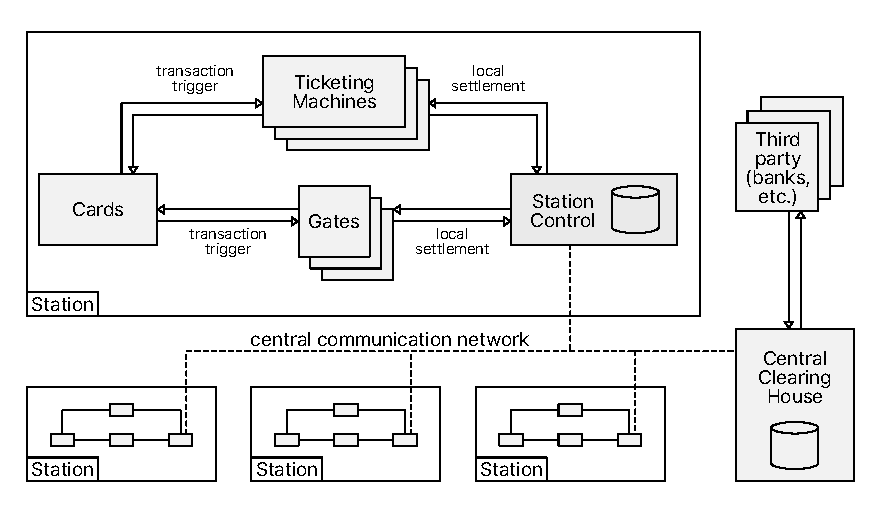
\includegraphics[width=.96\textwidth]{figures/tafc.pdf}
        \caption{Current AFC architecture}
        \label{f21currentaafc}
    \end{figure}
    
\subsection{Transaction Flow}
In general, two cases of fund transfer constitute transactions in AFC: card top-up and fare payment. Card top-up adds monetary value to account balance associated with the card spendable for transit fares. Fare payment consists of three major steps: entrance, exit, and settlement. Refer to Fig. \ref{f22currentaafc}. 

Beginning the trip, a passenger typically taps a transit card onto an RFID reader on an entrance gate. A computing device in the gate checks the card’s validity, including scrutinizing card number, the expiration, and the balance. Given that passenger taps a legitimate card, gate records the entrance both to the server’s metro data file and into the card, then opens the gate for passenger to begin the trip \cite{a6}. Upon exit, the exit gate performs identical validation and recording, calculates the fare based on fare structure, updates card balance inside the card and the server, then opens the gate \cite{a13}. Fund deduction and settlement are usually done offline to avoid users waiting too long for gate to open (i.e., more than 500 milliseconds \cite{a14}). Account balance reconciliation with central servers, in some rapid transit systems like Seoul Metro and the proposed San Diego Metro are done at the end of calendar day \cite{a13,a15}.

    \begin{figure}[H]
        \centering
        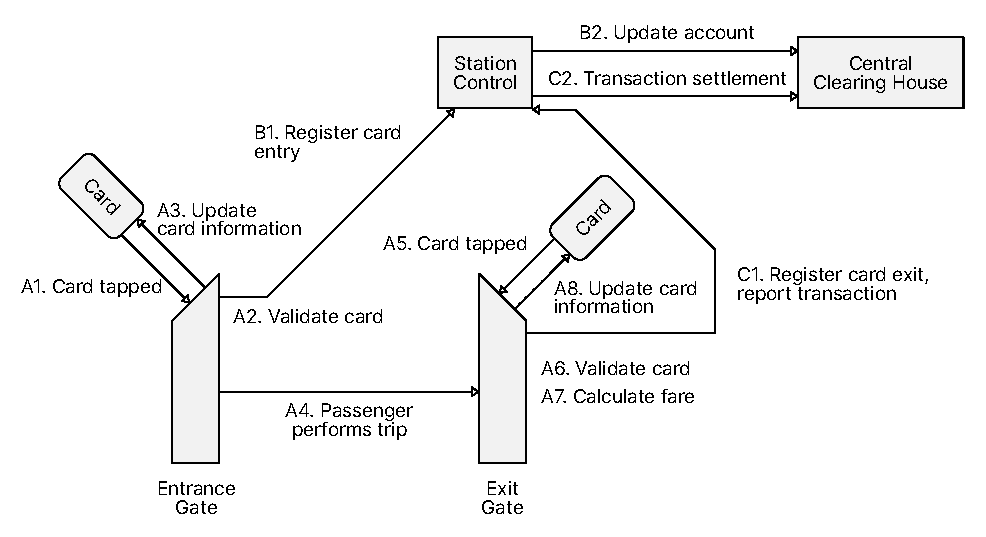
\includegraphics[width=.96\textwidth]{figures/tafc2.pdf}
        \caption{Current AFC transaction flow}
        \label{f22currentaafc}
    \end{figure}
    
In the United States, the American Public Transportation Association (APTA) sets out a proprietary standard AFC transaction format called the Contactless Fare Media Standard (CFMS). Allen et al. \cite{a17} recounts that APTA CFMS uses XML as its messaging protocol, in which they regard as highly resource consuming as it exceeds 350 milliseconds to complete one transmission. Some systems solve this problem by temporarily retaining at the edge to cope with latency or network unavailability \cite{a4} then settling the held transactions later at the central system.

\section{A Blockchain-based Toll Collection System for Public Sharing of Heterogeneous Edges \cite{a18}}

Xiao, et al. \cite{a18} examines the possibility of incorporating edge computing and blockchain in toll payment system called EdgeToll whose architecture and flow are illustrated in Fig. \ref{f23et} and \ref{f24et}. In EdgeToll, both toll users and provider use some cryptocurrency over blockchain to transact. When a user performs payment, he/she connects to a payment edge then pay the service fees at the edge. Later stage of EdgeToll includes a proxy which matches user-side and edge-side to reduce operational ‘gas’ costs by moving payment channeling off-chain.

	\begin{figure}[H]
        \centering
        \begin{subfigure}[b]{.44\textwidth}
            \centering 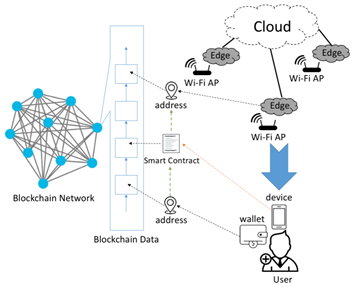
\includegraphics[width=0.99\linewidth]{figures/2-3.png}
            \caption{EdgeToll Architecture \cite{a18}}
            \label{f23et}
        \end{subfigure} 
        \begin{subfigure}[b]{.44\textwidth}
            \centering 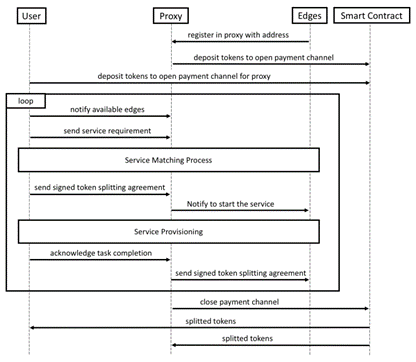
\includegraphics[width=0.99\linewidth]{figures/2-4.png}
            \caption{EdgeToll System Flow \cite{a18}}
            \label{f24et}
        \end{subfigure}
        \label{f2324}
    \end{figure}
    
\section{Blockchain-based Federated Learning for Edge Caching \cite{0a65}}
% ADD %%%%%%%%%%%%%%%%%%%%%%%%%%%%%%%%%%%%%%%%%%%%%%%%%%%%%%%%%%%%%%%%%%%%%
this work titled ""


\chapter{Background Knowledge}
\label{cbknowledge}

\section{Blockchain}
\subsection{Overview}
Blockchain is a growing peer-to-peer transaction record keeper in a form of a distributed ledger \cite{a7}. It equips encryption and stringent validation mechanisms in recording transactions and managing assets to ensure data integrity and security. As the name suggests, blockchain stores data in a form of blocks containing transaction details, hash of itself, and hash of the previous block, the latter used to make a linked list (‘chain’) of blocks (see Fig. \ref{f31}). Every party which participates in the network stores a copy of consensually agreed chain of blocks, hence the term “distributed ledger”.

    \begin{figure}[H]
        \centering
        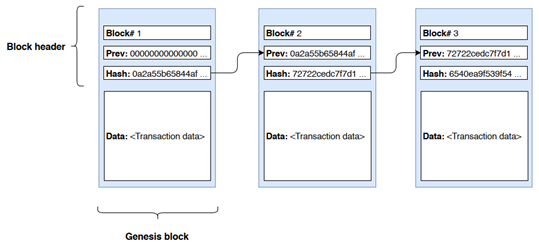
\includegraphics[width=.7\textwidth]{figures/3-1.png}
        \caption{Blockchain structure}
        \label{f31}
    \end{figure}
    
Blocks are compiled and proposed by network participants called “nodes”. Depending on the consensus mechanism, on pushing a block onto the chain, a node may have to perform a complex mathematical computation \cite{a7}. In Bitcoin’s Proof-of-Work (PoW) consensus, for instance, a node is given task to find a value which gives a hash beginning with a particular number of zeroes; the first node which finds one gains the right to append the chain with its proposed block then receives some incentive \cite{a20}. Once a block is added onto the chain, no one can modify its content except majority nodes agree on marking the validity of the modified block and its successor blocks. Therefore, such method of validation guarantees transaction correctness when honest nodes have more computational power than attacker nodes \cite{a7}. 

\subsection{Public, Private, and Permissioned Blockchain}

Bitcoin and most cryptocurrencies operate under blockchain concept, benefiting from its security, accountability, decentralization, and semi-anonymity: characteristics of public blockchains. Anyone can join and perform transactions on public blockchain networks without permission from a central authority. However, in intra-organizational use cases, conventional public blockchain suffers from a massive flaw: it requires a substantial amount of resource to confirm transactions and append them into a new block by performing challenges defined by its consensus protocol; besides, there is a need for data privacy in conducting business: public blockchains disallow such requirement.

Thus, there are types of blockchain networks that can accommodate privacy called private and permissioned blockchain. ‘Private’ and ‘permissioned’ blockchain, sometimes interchangeable, differ from public blockchain in several factors, namely: membership scope, and trust. Permissioned blockchain is mainly used in industries and businesses whose internal data needs to be transparent within a limited scope of parties. Only permissioned, white-listed nodes can participate in blockchain processes \cite{a21}; hence validating transactions needs not to be complex: by using Proof-of Authority (PoA) consensus approach. Contrary to PoW, in PoA, a node does not require any computational challenge to push a block onto a chain, rather, nodes selected by the authority of the blockchain can do so by proving its identity that shows the permission \cite{a5}. In this way, transaction speed is leveraged by much without compromising security factors.

\subsection{Smart Contracts}

Contracts are set of formal agreements between parties in conducting or establishing a relationship in personal, social, economic, and other fields. The agreements define roles, obligations, and rights of parties involved and determine actions to do in meeting a contract goal. Smart contracts are coded, automated contracts which are understandable by machines to run it with or without human intervention \cite{a22}.

Current applications of smart contracts lie around automated payments and asset transfer, which Nick Szabo declares them fit the nature of blockchain \cite{a23}. Not only regarding trade, but smart contracts also support credential and data logging, asset tracking, supply chain \cite{a23}, or even as a helper tool in judicial decision. Some blockchain projects such as Ethereum support smart contracts in a form of executable programs in blocks. One can tell a participant node to run a smart contract program by initiating a transaction which then invokes the program inside \cite{a24}.

\subsection{Decentralized Applications (dApps)}
To expand blockchain’s capability beyond transactional and contractual matters, Cai, et al. \cite{a24} claims that decentralized applications (dApps) hosted inside blockchain are the ideal blockchain application: applications whose operations are independent from human control. Cai, et al. gives example dApp projects, one being a smart hotel IoT system where guests do not have to interact with humans in renting a room: they just pay hotel fees into a smart contract, and a room is reserved for them automatically.

\section{Hyperledger \cite{a25}}
Hyperledger project, hosted by The Linux Foundation since 2015, is an open source blockchain project aimed to provide a blockchain framework for corporates and individuals to develop their own blockchain applications. Hyperledger follows five strict characteristics:
\begin{enumerate}
\item Modular: working blocks are reusable and will not affect other parts of the system when modified,
\item Highly secure: supported by openly reviewed protocols, algorithms, and cryptography,
\item Interoperable with other networks and platforms,
\item Independent from cryptocurrency: there will be no requirements of using tokens, and
\item User-accessible and transparent API.
\end{enumerate}

\subsection{Hyperledger Fabric \cite{a25,a26}}
Hyperledger Fabric is one of Hyperledger frameworks which focuses on deployment of modular distributed ledger for intra- and inter-industrial dApps. It follows a permissioned blockchain model where participants (peer and orderer nodes) are strictly appointed by a central network authority to reflect the management model in industries. Despite its strict access control mechanism, Hyperledger Fabric creates multi-channel network mechanism which enables stakeholders to segregate levels of shared information; as an illustration, when a company might want to share information about discounted prices to specific partners but not others, they can broadcast it in a separate channel from its main price-announcing channel. Refer to Fig. \ref{f32}. to view an example of Hyperledger Fabric’s system arrangement.

    \begin{figure}[H]
        \centering
        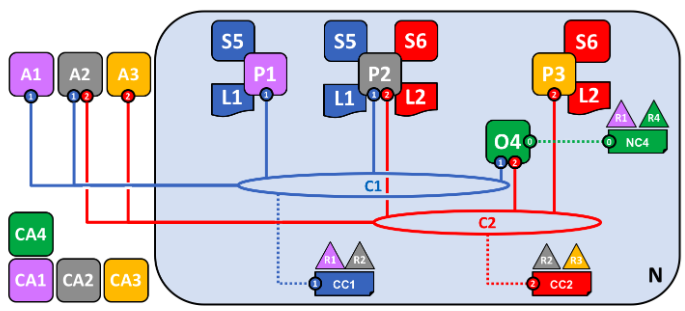
\includegraphics[width=.96\textwidth]{figures/3-2.png}
        \caption{Hyperledger Fabric Sample Network \cite{a26}}
        \label{f32}
    \end{figure}
    
Suppose four companies or entities share information with each other in a Hyperledger Fabric network $N$, namely $R1, R2, R3, and R4$. Imagine that $R4$ is the initiator of the network, thus $R4$ gains power to establish the first version of $N$ by introducing a network configuration $NC4$. In this scenario, $R1$ is appointed to be a co-curator of the network as well: it then governs $NC4$. $R4$ decides not to involve in business transactions in $N$; while $R1$ and $R2$ would like to have an exclusive communication channel between the two; as well as between $R2$ and $R3$. Therefore, $R1$ and $R2$ create and govern channel $C1$ and its configuration $CC1$. So do $R2$ and $R3$ with $C2$ and $CC2$. Each company $R1$, $R2$, and $R3$ then deploy their peer node, consecutively: $P1, P2,$ and $P3$. Since $R1$ and $R2$ share channel $C1$ with their peers $P1$ and $P2$, the peers keep a shared ledger $L1$ and smart contract $S5$; and ditto for $R2$ and $R3$ in channel $C2$. Note that because $P2$ belongs to channels $C1$ and $C2$, $P2$ keeps both $L1$ and $L2$ and can run $S5$ and $S6$. Transactions from any peer in $C1$ and $C2$ should be approved by ordering node $O4$ issued under $NC4$ before ledger change takes place. Next, suppose that each of $R1$, $R2$, and $R3$ wishes to deploy its own application $A1$, $A2$, or $A3$, the application will connect to their corresponding channel of choice. Finally, to prove organizational and component identities in a consensus mechanism, each company can define a certification authority ($CA$).

\subsection{China’s Blockchain-based Service Network (BSN) \cite{a8,a27}}
In 2019, The Government of People’s Republic of China initiated a national level blockchain platform rendered as Blockchain-based Service Network (BSN). It is an open Blockchain as a Service (BaaS) platform which allows blockchain developers from around the world to deploy dApps on, offering a complete set of development environment and resources. The network establishes public city nodes for developers to use for a low cost such that it would reach a wider customer target. BSN supports permissioned, permissionless, and interchain services; with Hyperledger Fabric as one of its supported permissioned blockchain platforms.

\subsection{Federated Learning}
%ABOUT FED LEARNING %%%%%%%%%%%%%%%%%%%%%%%%%%%%%%%%%%%%%%%%%%%%%%%%%%%%%%%%%%%%


\section{Methodology}
The research consists of two parts: (1) establishing and scrutinizing a blockchain-backed AFC system and (2) making use of data fed from blockchain for passenger caching.
\subsection{Part 1: Blockchain-backed AFC}
In this part, a blockchain-based AFC will be built in the following sequence:
\begin{enumerate}
\item Performing literature review on how AFCs are implemented through textual resources,
\item Obtaining smart card transaction dataset from an existing metro system,
\item Simulating the working of traditional AFC system and record its performance,
\item Constructing a novel AFC system, then
\item Comparing both systems’ performance and qualitative advantages and disadvantages.

The system to examine will consist of the following system blocks (tentative), see Fig. \ref{f33}:

\begin{enumerate}
\item Station control block, consisting of fare handling functions (control gates and top-up machines) as entities which initiate transactions. Several geographically proximate stations constitute a station agglomeration which connect to a common peer node,
\item Peer node creates and proposes new transactions from stations to the blockchain. Each peer node houses two Hyperledger components:
\begin{enumerate}
\item Smart contract contains transaction logic which will execute upon a transaction request. Smart contracts are written in Node.js (tentative),
\item Ledger: a copy of all transaction history from all stations and accounts, accompanied with a world state database,
\end{enumerate}
\item Channel: a communication grouping in which transaction data is shared with.
\begin{enumerate}
\item Private channel manages internal transaction records, and
\item Public channel contains limited information sufficient for the public to access, view, and use,
\end{enumerate}
\item Orderer node: a validator node which accepts and endorses the creation of new transaction block using Raft consensus and Crash-Fault Tolerance consensus. May be embedded in some stations or inside the pseudo-central clearing house,
\item Pseudo-central clearing house: a facility which accommodates node certification and identities of stakeholders of the system, and
\item Public applications: set of applications open for public to build upon the data provided in the public channel, which will not be implemented in this research,
\item Private applications: applications which serve internal business process such as station application (control gates, top-up machines) and in this research a dynamic pricing application which uses AFC data from the ledger to periodically control trip fares based on congestion level using Tensorflow.js deep learning library over Node.js.
\end{enumerate}

All blocks are under one integrated framework implemented in Linux’s Hyperledger Fabric. 

    \begin{figure}[H]
        \centering
        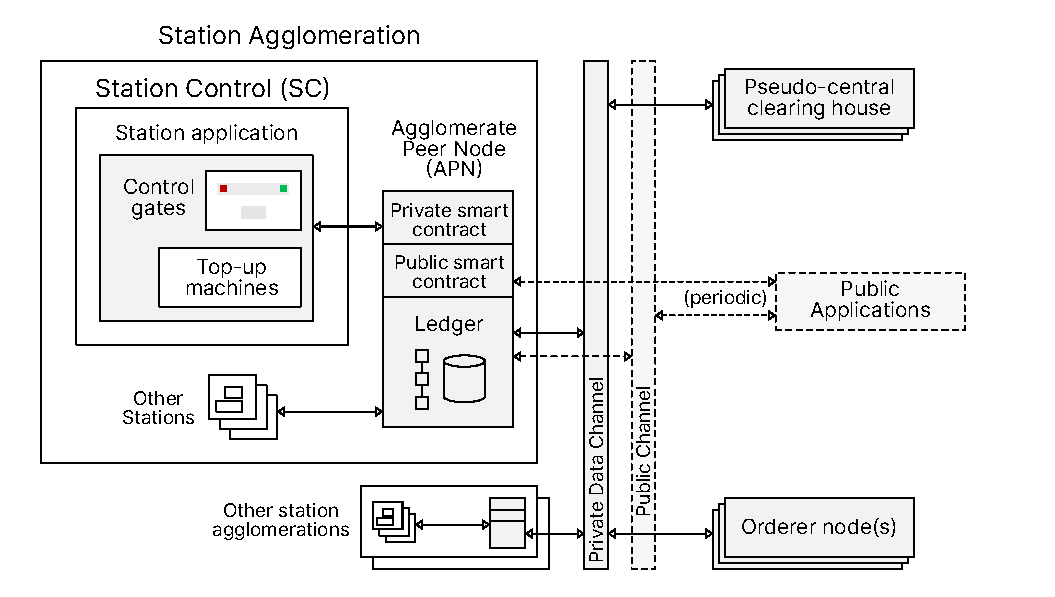
\includegraphics[width=.96\textwidth]{figures/bafc-main.pdf}
        \caption{Proposed AFC system}
        \label{f33}
    \end{figure}
    
Here, the dataset comes from smart card passenger transaction data of Shanghai Metro\footnote{Downloadable from https://pan.baidu.com/s/1w31Hldfiu7dGUkEpCYXIVg, accessed 2021.04.11} between 2015.04.01 to 2015.04.21 (around 280 million records). The .csv input data contains the categories in Table \ref{tdata}:

\begin{table*}[]
\caption{Sample metro data}
\tbl{}{
\label{tdata}
\begin{tabular}{p{0.15\linewidth}p{0.15\linewidth}p{0.11\linewidth}p{0.23\linewidth}p{0.07\linewidth}p{0.05\linewidth}p{0.09\linewidth}}
\textbf{Card Number} & \textbf{Transac. Date} & \textbf{Transac. Time} & \textbf{Station Name} & \textbf{Mode} & \textbf{Fare\footnotemark} & \textbf{Discount}\\ \hline
3000953650 & 2015-04-11 & 15:14:03 & 7号线肇嘉浜路 & 地铁 & 4 & 非优惠 \\ \hline
401456622 & 2015-04-11 & 09:45:42 & 2号线东昌路 & 地铁 & 7.2 & 优惠 \\ \hline
2802424753 & 2015-04-11 & 15:29:13 & 2号线上海科技馆 & 地铁 & 0 & 非优惠 \\ \hline
\vdots & \vdots & \vdots & \vdots & \vdots & \vdots & \vdots \\ 

\end{tabular}}
\end{table*}
\footnotetext{Shanghai metro fares follow the formula $price\_in\_yuan = 3 + \lceil (distance\_in\_km – 6) / 10 \rceil$. After cross-checking with Shanghai Metro fare calculator at http://service.shmetro.com/en/cphc (accessed on 2021.04.26), the prices still apply.}

Due to computing constraints, only a fraction of the whole data will enter the AFC system’s record. In an ideal case, recorded data in ledger would become a data source for the next part of the research: passenger caching; but, in this purpose, it is done just for the purpose of proving the work.

\subsection{Part 2: Blockchain-based Federated Learning (BFL)-assisted Caching}

Part 2 examines if the novel AFC can support a passenger caching mechanism to store frequent passengers' latest record in cache for faster data access. Federated Learning (FL) serves as the caching method. This subsystem uses another channel and smart contract set in Hyperledger Fabric. However, because of resource limitation, only a subset of the dataset is used.

Consulting Fig. \ref{f33a}, the caching system occupies another Hyperledger channel of the same network. Each station has a common cache

    \begin{figure}[H]
        \centering
        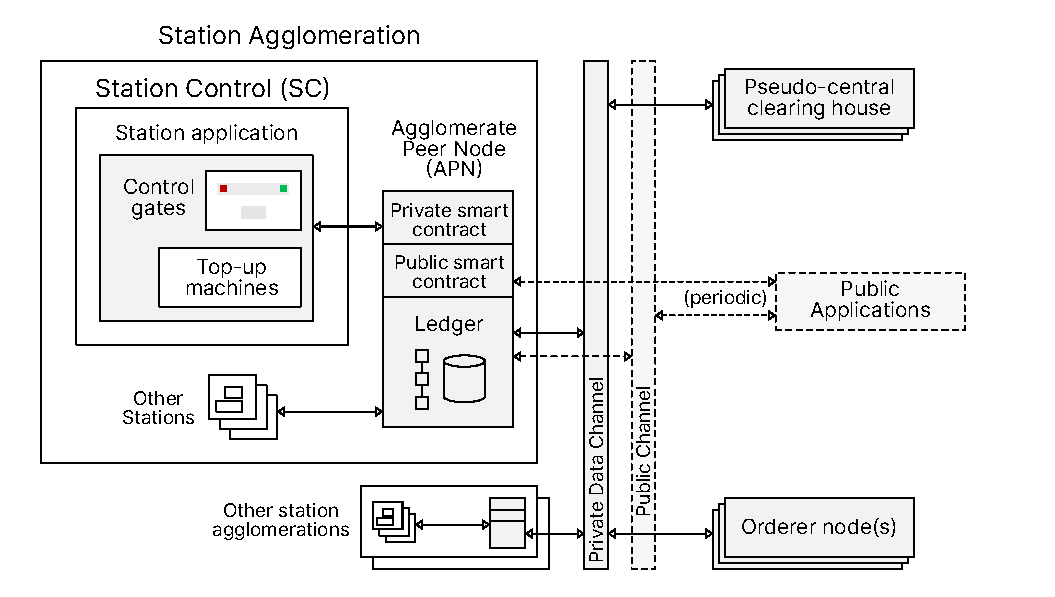
\includegraphics[width=.96\textwidth]{figures/bafc-main.pdf}
        \caption{Caching extension to the proposed AFC system: schematic}
        \label{f33a}
    \end{figure}

%steps



%further work: on buses (mobile BFL)



\DeclareFieldFormat{labelnumberwidth}{\textbf{[#1]}}
\printbibliography[heading=bibintoc,title={Bibliography}]
 
\begin{appendices}

\titleformat{\chapter}[display]{\bfseries\centering}{\LARGE Appendix \thechapter}{-0.5em}{\LARGE}

    \chapter{Appendix1}
        \label{appx:label1}
        appendix
\end{appendices}
\end{document}